\documentclass[11pt]{article}

% Packages
\usepackage{amsmath}
\usepackage{graphicx}
\usepackage{amssymb}
\usepackage{longtable}
\usepackage[spanish]{babel}
\usepackage[utf8]{inputenc}
\usepackage[T1]{fontenc}
\usepackage{float}


\author{Brian Ameht Inclán Quesada C-411\\ Davier Sánchez Bello C-412\\ Eric López Tornas C-411}
\title{Proyecto Final de IA y Simulación \\ Juego de Supervivencia}
\date{}

% Document
\begin{document}

\maketitle
\newpage

\tableofcontents
\newpage

\section{Introducción}
Sugarscapes, expuesto extensamente en el libro "Growing Artificial Societies", publicado en 1996 bajo la autoria de Joshua Epstein y Robert Axtell es un modelo de simulacion clasico, que a traves de una simulacion bastante simple, con agentes de un comportamiento muy sencillo y pocos rasgos a modelar, logra simular con resultados muy realistas los comportamientos de las sociedades humanas en cuanto a distribucion de la riqueza, transmision cultural, reproduccion, combates, entre otros.
En SugarScapes, los agentes carecen de una verdadera IA detras de si, y son mas bien homogeneos a pesar de sus diferentes rasgos, debido a que todos actuan de manera similar en la mayor parte de las simulaciones inspiradas en SugarScapes.
Nosotros, quisimos explorar el tema de la violencia y la formacion de agrupaciones (bandas de gangster y demas) en la socieda, a traves de nuestra propia version de SugarScapes, pero cargando a los agentes de un comportamiento basado en IA. Queremos estudiar cuanto influyen el rango de vision, de movimiento, la riqueza heredada por un agente, su nivel de consumo, asi como la zona en que nacion en su supervivencia en un ambiente donde la reparticion de los recursos naturales que aparecen distribuidos de manera desigual esta signada por la ley del mas fuerte, por la violencia. Asi, algunos agentes eligiran asociarse a otros, bajo ciertas reglas de asociacion, mientras otro eligiran huir de los conflictos todo el tiempo y otros provocarlo. Cual de estas estrategias es mejor, es mejor la misma para cada tipo de agente en cuando a su capacidad de vision, movimiento y herencia, o para cada nivel de capacidad hay una estrategia que mas probablemente le asegure la supervivencia. Estas y otras preguntas que nos plantearemos son facilmente extrapolables, al igual que nuestra simulacion, a situaciones de la vida real, donde los individuos deben agruparse para tener mas fuerza y/o ejercerla sobre los demas, para sobrevivir, o inlcuso alcanzar mas poder.

\section{Modelo}
\subsection{Resumen del modelo}
Emparentado a Sugarscapes, nuestro modelo consiste en una grilla bidimensional, donde conviven diferentes tipos de agentes. Cada agente ocupa una casilla de la grilla, y cada casilla puede soportar una cantidad maxima de azucar, que varia para cada una. Todos los turnos las casillas que no han alcanzado su maximo potencial de azucar, incrementan en 1, aunq este parametro es ajustable, la cantidad de azucar que contienen. Cada vez que los agentes visitan una casilla, recogen todo el azucar presente en esta, e incrementan sus reservas en la cantidad de azucar recogida. Deben, todos los turnos, satisfacer su necesidad diaria de azucar, consumiendo sus propias reservas. Si en algun momento sus reservas caen de 0, mueren.
Los agentes podran interactuar entre si atacandose o haciendo asociaciones. Una asociacion es un pacto entre dos o mas agentes donde cada uno acuerda ceder un determinado por ciento de sus ganancias a la asociacion y luego a cada cual le corresponde una porcion de las ganancias totales de la asociacion. Pudieran ademas implementarse otras formas de relaciones sociales como las extorsiones.
Los agentes tendran diferentes rangos y formas de movimientos, de vision y de ataques, asi como naceran con diferentes necesidades de consumo y reservas.
\subsection{Ventajas}
La principal ventaja de este modelo de simulacion es que incluso tras introducir IA a los agentes y complejizar sus relaciones, la simulacion sigue siendo lo suficientemente simple como para incorporar un volumen considerable de agentes, de diferentes tipos, y correr un volumen suficiente de simulaciones como para llegar a conclusiones. Otra ventaja de este modelo es que, estando basado en la experiencia previa del Sugarscapes, sabemos y podemos comprobabr que emula muy bien los fenomenos ocurridos en la tan compleja sociedad humana, partiendo de una simulacion muy sencilla
\subsection{Desventajas}
La principal desventaja que encontramos en este modelo para estudiar las agrupaciones de violencia en las sociedades humanas es que no toma en cuenta la compatibilidad de caracter entre los agentes, o sea, todos los agentes pueden tener el mismo tipo de relaciones con todos los demas agentes. En la vida real, el caracter de algunas personas sles hace mas dificil e incluso imposible mantener algun tipo de relacion con otras personas, mientras que facilita el acercamiento entre otras. El modelo descrito realmente no toma en cuenta esta arista tan importante del factor humano.
\subsection{Posibles mejoras}
Respecto a la desventaja presentada anteriormente, se pudieran evaluar para incrementar en cuanto a realismo la simulacion, ciertas soluciones propuestas precisamente en el libro Growing Artificial Societies. En tal libro, se logra modelar caracteristicas culturales de los individuos como cadenas de bits donde ciertas propiedades de la cadena, ya fuera la posicion de los bits encendidos y apagados o la cantidad total de tales bits, sirven para agrupar a los agentes en diferentes categorizaciones, y sirven como su diferenciador cultural. Muy bien podriamos emplear esta variante para simular el caracter de los agentes y determinar cuales tienen relaciones mas fluidas con otros, lo cual pudiera ser un factor para retrasar sus comunicaciones, o que influya en sus tomas de decisiones.
Otra mejora que se pudiera hacer a la simulacion, y que parece obvia dado el tema escogido, es la introduccion de relaciones familiares entre los agentes, de manera que, al avanzar la simulacion, los clanes terminarian nucleando a una o unas pocas familias cada uno, y las relaciones familiares se convirtieran en un medio de poder, tal y como sucede en las agrupaciones mafiosas y las bandas violentas que intentamos emular.
Hablo aqui acerca d lo q nos falto hacer?

\section{Implementación}
\subsection{Modelo de la simulación}
\subsection{Agentes}
En nuestra simulación de supervivencia, utilizamos varios tipos de agentes, cada uno con estrategias y objetivos específicos que influyen en su comportamiento dentro del juego.Todos tienen un sistema experto que emula el conocimiento y la toma de decisiones del agente,
basandoce en la información que se le proporciona en el entorno de juego. Estas desiciones se toman en dependencia de las regls que se definan en el sistema experto, más explicado adelante. A continuación, describimos los tipos de agentes que utilizamos en nuestra simulación:

\subsubsection{Agente Aleatorio (RandomAgent)}
El \textit{RandomAgent} actúa sin una estrategia fija, moviéndose de manera aleatoria en el tablero. Este agente no busca activamente comida ni evita el combate, lo que lo hace impredecible y a menudo vulnerable a ataques.

\subsubsection{Agente Pacífico (PeacefulAgent)}
El \textit{PeacefulAgent} busca evitar conflictos a toda costa. Su estrategia principal es alejarse de los agentes de combate y buscar rutas que lo mantengan distante de posibles amenazas. Este agente también intenta encontrar recursos, pero prioriza su seguridad sobre la acumulación de los mismos.

\subsubsection{Agente de Combate (CombatAgent)}
El \textit{CombatAgent} está diseñado para la confrontación. Su objetivo es localizar y atacar a otros agentes. Utiliza un algoritmo de búsqueda, como BFS o A*, para planificar su ruta hacia el agente más cercano o estratégicamente importante. Es agresivo y busca maximizar el daño a los oponentes mientras minimiza su propia exposición al peligro.

\subsubsection{Agente Inteligente (SmartAgent)}
El \textit{SmartAgent} utiliza algoritmos avanzados de toma de decisiones y aprendizaje automático para adaptar su comportamiento basado en la dinámica del juego. Este agente evalúa constantemente el estado del juego, tomando decisiones informadas sobre cuándo recolectar recursos, combatir, o retirarse basado en las probabilidades de éxito y supervivencia.

\subsubsection{Agente Buscador de Comida (FoodSeekerAgent)}
El \textit{FoodSeekerAgent} se centra principalmente en la búsqueda de recursos alimenticios. Utiliza algoritmos de búsqueda para encontrar el camino más eficiente hacia las áreas con alta densidad de recursos. Aunque evita el combate, está diseñado para tomar rutas óptimas que balanceen la adquisición de comida y la evasión de amenazas.

\paragraph{Ejemplo de Implementación del Agente Buscador de Comida}
En el siguiente ejemplo, ilustramos cómo un \textit{FoodSeekerAgent} opera en un tablero de \(10 \times 10\) buscando la ruta más segura hacia áreas ricas en recursos. La posición inicial del agente es \( (0, 8) \) y se mueve hacia \( (2, 9) \), identificada como la región con mayor disponibilidad de comida, evitando encuentros hostiles.

\subsection{Base de conocimiento y toma de decisiones}
Este sistema se basa en una estructura modular que integra hechos y reglas dentro de un motor de inferencia para gestionar y tomar decisiones basado en conocimientos. Está diseñado para funcionar en entornos donde las decisiones se toman a partir de un conjunto de datos dinámico y posiblemente en tiempo real. Los componentes clave son:

\begin{itemize}
    \item \textbf{Enumeración \textit{Knowledge}:} Es una enumeración que define diferentes tipos de conocimientos que pueden ser importantes en un contexto de toma de decisiones. Estos incluyen aspectos como la posición, la salud, los ataques disponibles, las asociaciones y más. Cada tipo de conocimiento sirve como una clave que identifica un tipo de información específica dentro del sistema
    \item \textbf{Clase \textit{Fact}:}  Representa un hecho o una pieza de información en el sistema. Cada hecho está compuesto por una clave (un valor de Knowledge) y un dato asociado a esta clave. Esta estructura permite almacenar y gestionar información dinámica que el sistema utiliza para tomar decisiones
    \item \textbf{Clase \textit{Rule}:}  Define una regla en el sistema, la cual consta de una condición y una acción. La condición es una función que toma un conjunto de hechos y determina si la regla debe ejecutarse. Si la condición es verdadera, la acción (también una función) se ejecuta para generar nuevos hechos basados en los hechos existentes. En resumen, esta clase permite definir la lógica del sistema para generar nuevos hechos a partir de los existentes.
    \item \textbf{Clase \textit{BaseKnowledge}:} Esta clase especifica las operaciones fundamentales para cualquier sistema de conocimiento, como aprender y tomar decisiones.
    \item \textbf{Clase \textit{Estrategy}:} Es una implementación concreta de BaseKnowledge. Gestiona un conjunto de hechos y reglas a través de un motor de inferencia. Permite añadir y eliminar conocimientos y reglas, aprender de nuevos datos y tomar decisiones basadas en las reglas definidas y los hechos actuales
    \item \textbf{Clase \textit{InferenceEngine}:} Es el componente que realiza la inferencia lógica. Gestiona un conjunto de hechos y reglas, permitiendo añadir y eliminar estos elementos. El método run de InferenceEngine es crucial: evalúa todas las reglas con los hechos actuales para generar nuevos hechos, los cuales pueden influir en decisiones futuras.
\end{itemize}

Este modelo permite un manejo flexible y dinámico de información, esencial para la toma de decisiones en entornos cambiantes, tal y como necesitamos en nuestra simulacion.
\subsection{Algoritmos de búsqueda}
En esta sección, describiremos varios algoritmos de búsqueda utilizados en nuestro proyecto. Cada algoritmo será tratado en una subsección independiente, donde se explicará su funcionamiento, particularidades y ejemplos de uso.

\subsubsection{Algoritmo A*}
El algoritmo A* es una técnica de búsqueda de camino que encuentra el camino más corto entre un nodo inicial y un nodo objetivo en un grafo. Utiliza una combinación de costos conocidos para llegar a un nodo \( g(n) \) y una estimación heurística \( h(n) \) del costo para alcanzar el objetivo desde ese nodo. La función \( f(n) = g(n) + h(n) \) guía el algoritmo para explorar los caminos más prometedores primero.

En nuestro caso estamos implementado usando una estructura de tipo $min-heap$, denominada $open\_heap$. Esta estructura se utiliza para mantener los nodos que aún necesitan ser explorados en el algoritmo. Mediante un heap de minimos organiza los elementos de tal manera que el primer elemento es siempre el más pequeño, lo cual es útil para extraer rápidamente el nodo con el costo estimado más bajo para continuar la búsqueda.


\paragraph{Detalles del Funcionamiento}
\begin{itemize}
    \item \textbf{Heurística}: La función heurística es crucial en A*. Una elección común es la distancia Manhattan, útil en grillas donde solo se permiten movimientos horizontales y verticales.
    \item \textbf{Conjunto de abiertos}: A* mantiene un conjunto de nodos conocidos como el "conjunto abierto". Inicialmente, contiene solo el nodo de inicio.
    \item \textbf{Bucle Principal}: En cada paso del algoritmo, el nodo con el menor valor de \( f(n) \) se retira del conjunto abierto. Este nodo es procesado considerando todos sus nodos vecinos. Para cada vecino, se calcula \( g(n) \) y \( h(n) \), y si el nuevo camino es mejor, se actualiza el camino.
\end{itemize}

\paragraph{Ejemplo de Uso}
En el siguiente ejemplo mostramos un agente del tipo $FoodSeekerAgent$ que en nuestra simulacion representa al agente que esta constantemente buscando la mejor manera de llegar al lugar donde mas recursoa halla. En este caso tenemos un tablero de \(10 \times 10\). Definimos la posición inicial como \( (0, 8) \) y el objetivo en este caso la casilla que dentro de su rango de vision
es la que mas recursos posee, como \( (2, 9) \). La salida del algoritmo proporcionará la secuencia de movimientos para llegar del inicio al objetivo, evitando los obstáculos, que en este ejemplo no hay ninguno.

\begin{figure}[H]
    \centering
    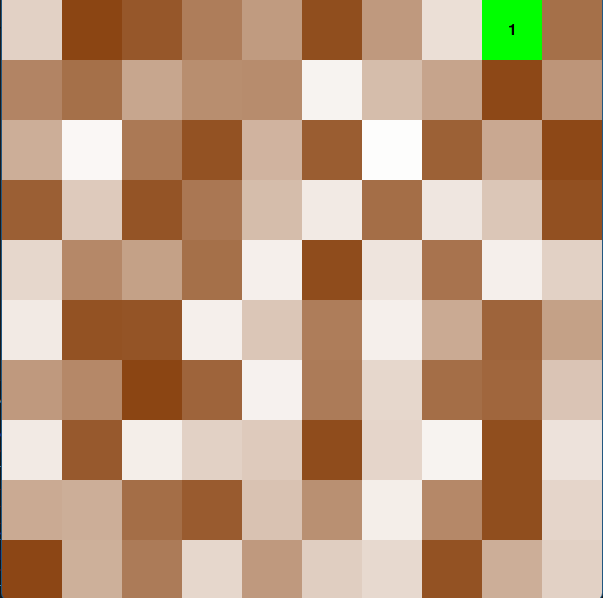
\includegraphics[width=0.18\textwidth]{images/image1.png}\hfill
    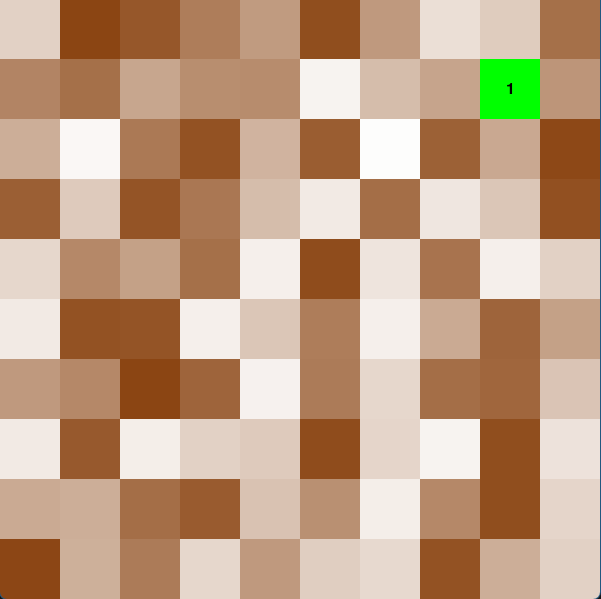
\includegraphics[width=0.18\textwidth]{images/image2.png}\hfill
    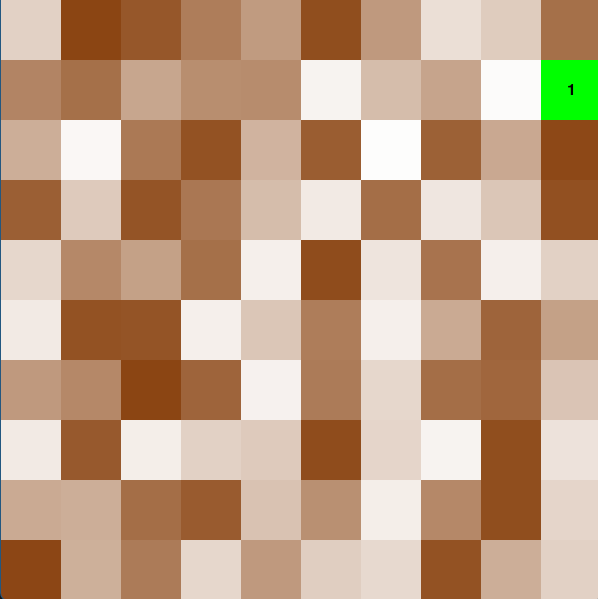
\includegraphics[width=0.18\textwidth]{images/image3.png}\hfill
    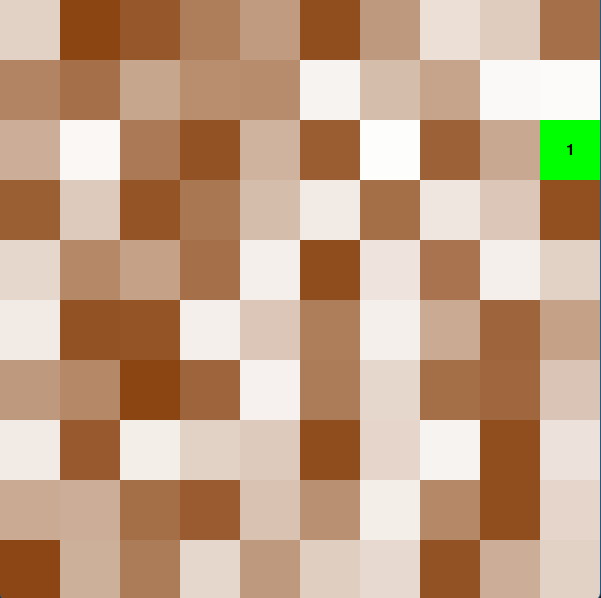
\includegraphics[width=0.18\textwidth]{images/image4.png}
    \caption{Secuencia de movimientos del agente FoodSeekerAgent en la simulación desde la posicion \( (0, 8) \) hasta \( (2, 9) \) .}
\end{figure}

\paragraph{Implementación}
Para implementar el A* en la simulación de nuestro juego, utilizamos una clase que gestiona la verificación de movimientos válidos y obstáculos. Esta clase ajusta el algoritmo para adaptarse a las características específicas del entorno de juego, como áreas inaccesibles y diferentes costos de movimiento asociados con diversos tipos de terreno.

\subsubsection{Búsqueda en Amplitud (BFS)}
La Búsqueda en Amplitud, o BFS por sus siglas en inglés (Breadth-First Search), es un algoritmo clásico para explorar grafos y árboles. Es especialmente útil en situaciones donde necesitamos encontrar el camino más corto en términos de número de aristas entre un nodo de origen y otros nodos, dado que explora todos los nodos a la misma profundidad antes de moverse a la profundidad siguiente.
En nuestra simulación está especialmente diseñado para calcular rutas de escape en situaciones donde un agente necesita maximizar la distancia de un atacante en un entorno de grilla. La adaptación permite a los usuarios elegir entre obtener sólo el siguiente movimiento óptimo o el camino completo de escape.

\paragraph{Funcionamiento de BFS}
La implementación de BFS comienza con la inserción del nodo de origen en una cola. A medida que cada nodo se procesa, sus vecinos no visitados se añaden al final de la cola. Este proceso continúa hasta que se visitan todos los nodos alcanzables o hasta que se encuentra el nodo objetivo, lo que permite una exploración completa en capas.

\begin{itemize}
    \item \textbf{Cola de BFS}: Utilizamos una cola para mantener el orden de exploración de los nodos. En nuestra implementación, esto se maneja con una estructura de datos deque para una eficiente inserción y eliminación de elementos.
    \item \textbf{Conjunto de Obstáculos y Visitados}: Mantenemos un conjunto de obstáculos para evitar la exploración de nodos no transitables y un conjunto de nodos visitados para evitar procesar el mismo nodo más de una vez.
    \item \textbf{Validación de Movimientos}: Cada movimiento potencial se valida para asegurar que no se salga del límite del entorno de juego y no se encuentre con obstáculos.
\end{itemize}

\paragraph{Ejemplo de Uso}
En el siguiente ejemplo, mostramos un agente del tipo $PacifistAgent$ \( (azul) \) en la posicion \( (5, 6) \), que en nuestra simulación representa al agente que tiene una estrategia pacifica, evade los ataques e intenta sobrevivir.
En este caso, tenemos un tablero de \(7 \times 7\). Definimos la posición inicial del agente $CombatantAgent$ \( (rojo) \) como \( (3, 3) \). La salida del algoritmo proporcionará la secuencia de movimientos para llegar a la posición segura más lejana posible, evitando al atacante, evidenciamos en las siguientes imagenes como
la secuencia de movimientos incluye como primer movimiento el de alejarce del atacante hacia la casilla \( (6, 6) \), luego en el siguiente movimiento, este se queda en esa misma posicion ya que de entre las posibles es la mas lejana al atacante


\begin{figure}[H]
    \centering
    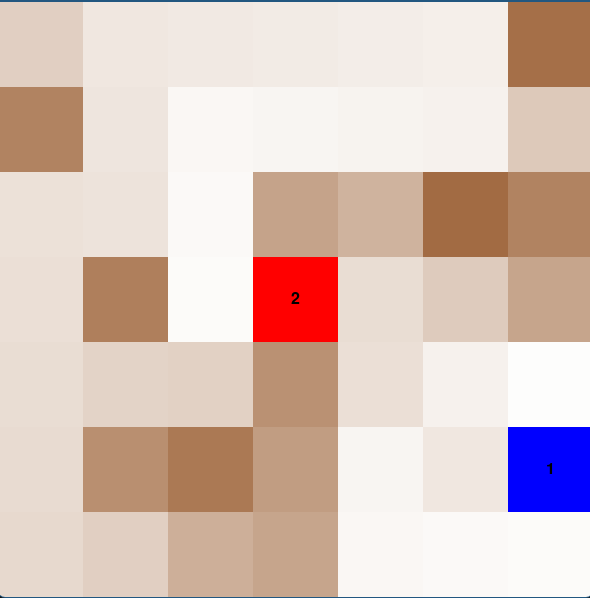
\includegraphics[width=0.18\textwidth]{images/image6.png}\hfill
    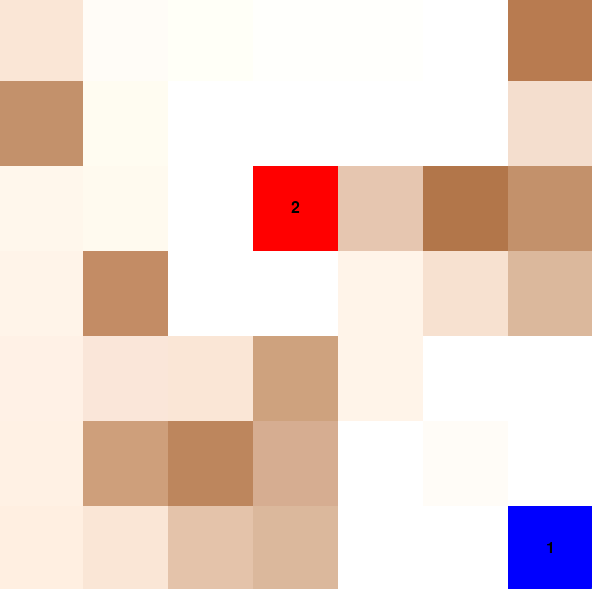
\includegraphics[width=0.18\textwidth]{images/image7.png}\hfill
    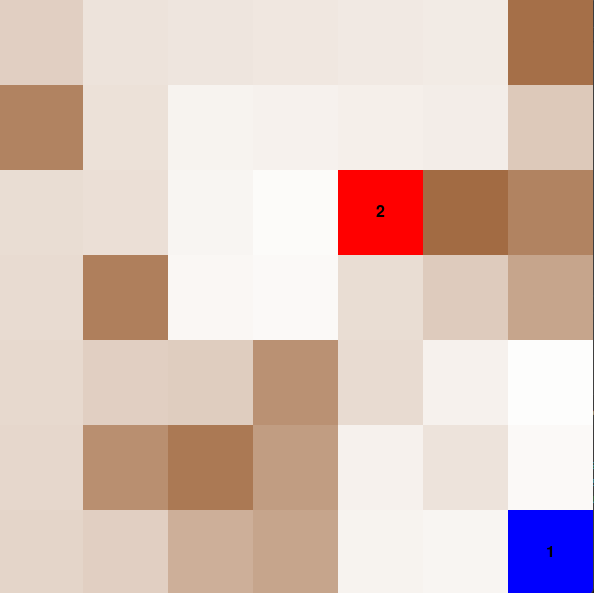
\includegraphics[width=0.18\textwidth]{images/image8.png}
    \caption{Secuencia de movimientos calculada por BFS para evadir al atacante, mostrando cada paso desde el inicio hasta la posición segura más lejana posible.}
\end{figure}

\paragraph{Implementación}
Nuestra clase \textit{BFS} incluye métodos para configurar los obstáculos y calcular la ruta basada en las posiciones dinámicas de los agentes y las barreras en el entorno. Esto asegura que el agente siempre tenga una ruta de escape actualizada y pueda reaccionar a los cambios en el entorno.



\subsubsection{Monte Carlo Tree Search (MCTS) (Trabajo en proceso)}
El Monte Carlo Tree Search (MCTS) es un algoritmo de búsqueda heurística ampliamente utilizado en la toma de decisiones en juegos y problemas de optimización combinatoria. A diferencia de otros enfoques, como la búsqueda en profundidad, MCTS no requiere un conocimiento completo del espacio de búsqueda y es especialmente útil en entornos con una gran cantidad de acciones posibles y una complejidad elevada.\\

Este método se basa en una búsqueda inteligente de árboles que equilibra la exploración y la explotación. Utiliza el concepto de muestreo aleatorio mediante simulaciones, conocidas como "playouts", para evaluar las diferentes opciones disponibles. A medida que se realizan más playouts, el algoritmo acumula estadísticas sobre las acciones tomadas.\\

En nuestra implementación, aplicamos MCTS para guiar al agente en la selección de acciones óptimas en un entorno simulado. Consideramos el limitado conocimiento del usuario sobre la simulación para adaptar la exploración del árbol de búsqueda y priorizar aquellas acciones que parecen más prometedoras según las heurísticas de comportamiento implementadas en los agentes.\\

\paragraph{Funcionamiento de MCTS}
Cada vez que un agente emplea MCTS en la toma de decisiones, se crea un objeto MCTS que representa el árbol de búsqueda del agente en ese turno. La raíz de este árbol refleja el estado de la simulación justo antes de que el agente tome una decisión. El algoritmo de MCTS sigue un ciclo de cuatro pasos:\\

\begin{itemize}
\item \textbf{Selección}: Desde el nodo raíz R, se busca un nodo hoja L que represente un escenario de la simulación desde el cual no se ha tomado ninguna decisión. 
\item \textbf{Expansión}: A menos que el nodo L sea terminal (es decir, el agente gana o pierde), se expande el árbol de búsqueda creando uno o más nodos secundarios. Estos nodos representan movimientos válidos desde la posición de juego definida por L.
\item \textbf{Simulación}: Se realiza una reproducción aleatoria del juego desde el nodo C, elegido durante la fase de expansión. Esta simulación proporciona una estimación del valor de ese nodo y ayuda a evaluar la calidad de las acciones disponibles.
\item \textbf{Actualización}: El resultado de la simulación se utiliza para actualizar la información en los nodos de la ruta desde C hasta R, lo que permite al algoritmo ajustar sus estimaciones y mejorar la toma de decisiones futuras.
\end{itemize}

\paragraph{Implementación}
En nuestra implementación de MCTS, aprovechamos la información observada por el agente y su conocimiento previo de la simulación, como los agentes que ha visto cercanos o el recuento global de muertes, para construir una representación simplificada del escenario.

\paragraph{Ejemplos}
Ejemplos...



\subsection{LLM}
Utilizamos el LLM para la creación de agentes y la configuración del escenario de la simulación, así como para la función de comentarista del juego. Para la creación de agentes, empleamos una lista con descripciones por defecto de los comportamientos de nuestros tipos de personajes y la información suministrada por el usuario. El LLM infiere cuál es el tipo de personaje por defecto que más se acerca a la descripción del usuario, así como las estadísticas, teniendo en cuenta la mención u omisión de aspectos positivos y negativos en la descripción del personaje.
\\
En cuanto a la creación del mapa, se eligen las dimensiones del escenario a simular de acuerdo a la inferencia realizada por el LLM en la descripción del terreno.  \\
Para la función de comentarista, alimentamos al LLM con las últimas acciones ocurridas en la simulación y las descripciones de los personajes. Esto permite al modelo crear un breve relato de los eventos más recientes no comentados en la simulación.
\subsection{Interfaz de la simulación}

\section{Análisis de la simulación}
\section{Conclusiones}

\end{document}
